%%%%%%%%%%%%%%%
% This file is concerned with the interaction diagram.
%
% Please remember to compile the document from "00_finalreport.tex".
% It will not work otherwise.
%%%%%%%%%%%%%%%

\section{Interaction Diagrams}
	
	\subsection{Navigates to System}
	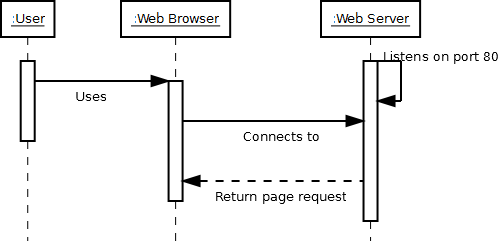
\includegraphics[width=0.50\textwidth]{./Interact1.png}
	
	This is a low coupling principle. The user uses their web browser which then interacts with our web server to display any information we intend to send.
	
	\subsection{Select Game}
	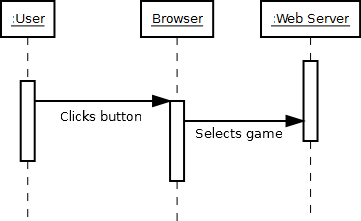
\includegraphics[width=0.50\textwidth]{./Interact2.png}
	
	Same principle as above. The user slects a game.
	
	\subsection{Connects}
	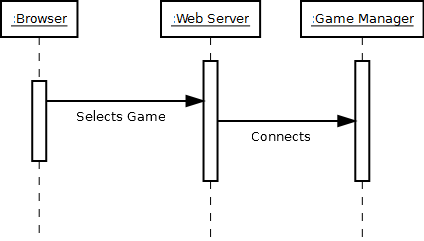
\includegraphics[width=0.50\textwidth]{./Interact3.png}
	
	High cohesion, The web server only deals with sending info to the browser, the game manager is responsible for all else.
	
	\subsection{Relays game selection}
	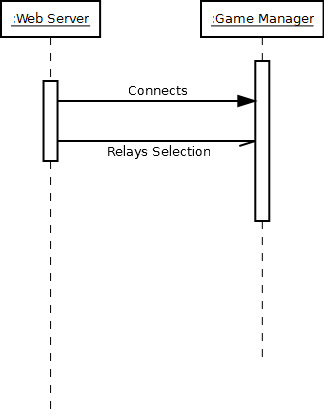
\includegraphics[width=0.50\textwidth]{./Interact4.png}
	
	This would full under the controller principle. Web server connected to the game manager and then passed alone the information that game manager needs to continue.
	
	\subsection{Provides information}
	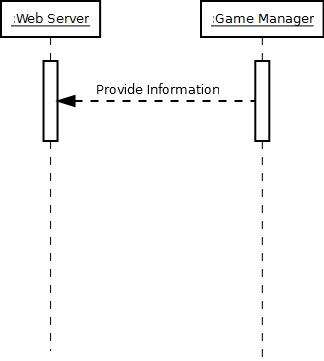
\includegraphics[width=0.50\textwidth]{./Interact5.png}
	
	Game manager provides the requested information to the web server to pass alone to user.
	
	\subsection{Interpret}
	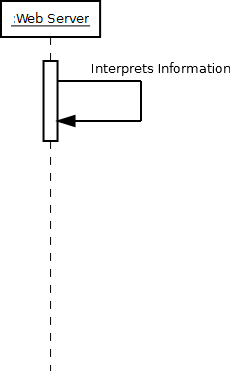
\includegraphics[width=0.50\textwidth]{./Interact6.png}
	
	It is now the web servers job to interpret the data that was passed to it.
	
	\subsection{Display}
	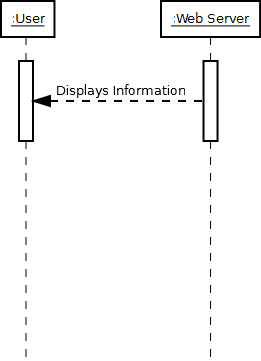
\includegraphics[width=0.50\textwidth]{./Interact7.png}
	
	Web server sends the translated information to the users browser to be displayed.
	
	\subsection{Close}
	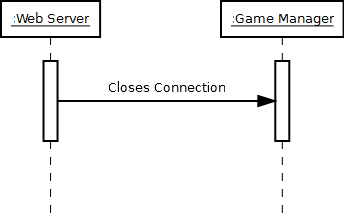
\includegraphics[width=0.50\textwidth]{./Interact8.png}
	
	The task is complete so the web server closes the connetion to the game manager.
	
	\subsection{Inform}
	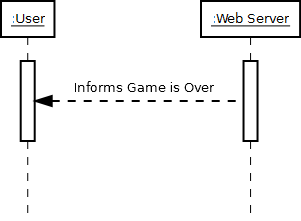
\includegraphics[width=0.50\textwidth]{./Interact9.png}
	
	Web server tells the user it has closed game session.

\newpage
